\NeedsTeXFormat{LaTeX2e}
\documentclass{jfp}
\usepackage{amssymb}
\usepackage{xcolor}
\usepackage{semantic}
\usepackage{comment}

\begin{comment}
Dear editors,
I'm grateful to the reviewers for their thorough assessment of the paper. I was very happy to read that the reviewer #2 perfectly captured my hope for the paper ("I must confess that at first Compost seemed too simplistic---but upon reflection I realize that is rather the point"), but the reviewers 1 and 3 made a number of excellent points that deserved clarification. I made a number of changes in response to the reviews.

MAJOR CHANGES
The following two major additions should clarify the paper w.r.t. many of the points made by reviewer 1 about the language design and its expressive power and limitations, as well as to answer points made by other reviewers (Haskell Chart, pie charts):

* I added a new section 2.3 (Choosing the level of language abstraction) which provides more background on the design of the DSL and contrasts it with Haskell Chart library and the Pan language. This should address the concerns of reviewer 1 and explain that, e.g. supporting combinators like "above s1 s2" was not the intention of the design.

* I added a new section 7 (Limitations and further work) that documents some of the things that are currently not supported. This discusses issues such as Pie charts (mentioned by reviewers 1 and 3), logarithmic and contracted axes (reviewer 3) and also visual aspects (reviewer 3). The section explains what is "not yet implemented" vs. what is "not supported by design".

MINOR CHANGES
The following are the notable minor changes that directly address the more specific reviewer comments:

* Reviewer 1 asked for clarification re "nest" - the explanation has been extended to be more clear
* Reviewer 2 pointed out a number of typos - all have been fixed (Thank you!)
* Reviewer 2 asked about figure placement - I tried to improve this (but sometimes unsuccessfuly as I also want to keep long code snippets on one page)
* Reviewer 3 asked about tight links with F# and Elm - I extended the discussion of implementation at the end of Section 1
* Reviewer 3 asked for clarification of syntactic categories in Figure 3 - this is now done.
* Reviewer 3 asked about syntax of host language vs. DSL - this is now explained at the start of Section 2.2
* Reviewer 3 asked about units of measure - I believe this is covered in Section 2.5 (in the context of types)
* Reviewer 3 asked for clarification re interaction - I added new paragraph in Section 5 and also made changes throughout to answer other specific questions raised

\end{comment}





\title{Composable data visualizations}
\author[Tomas Petricek]{TOMAS PETRICEK\\
       University of Kent, UK\\
       \email{t.petricek@kent.ac.uk}}

\definecolor{kvdclr}{rgb}{0.5,0.0,0.5}
\definecolor{fkvdclr}{rgb}{0.0,0.0,0.6}
\definecolor{urlclr}{rgb}{0.0,0.0,0.8}
\definecolor{idclr}{rgb}{0.0,0.0,0.0}
\definecolor{numclr}{rgb}{0.0,0.4,0.0}
\definecolor{strclr}{rgb}{0.6,0.2,0.0}

\newcommand{\X}{\emph{x}\ }
\newcommand{\Y}{\emph{y}\ }
\newcommand{\lsep}{\;\;|\;\;}
\newcommand{\num}[1]{\textcolor{numclr}{#1}}
\newcommand{\str}[1]{\textnormal{\textcolor{strclr}{\sffamily "#1"}}}
\newcommand{\strf}[1]{\textnormal{\textcolor{strclr}{\sffamily #1}}}
\newcommand{\ident}[1]{\textnormal{\textcolor{idclr}{\sffamily #1}}}
\newcommand{\kvd}[1]{\textnormal{\textcolor{kvdclr}{\sffamily #1}}}
\newcommand{\fkvd}[1]{\textnormal{\textcolor{fkvdclr}{\sffamily #1}}}
\newcommand{\narrow}[1]{\hspace{-0.6em}#1\hspace{-0.6em}}
\newcommand{\urrl}[1]{\textnormal{\textcolor{urlclr}{#1}}}

\newcommand{\langl}{\begin{picture}(4.5,7)
\put(1.1,2.5){\rotatebox{60}{\line(1,0){5.5}}}
\put(1.1,2.5){\rotatebox{300}{\line(1,0){5.5}}}
\end{picture}}
\newcommand{\rangl}{\begin{picture}(4.5,7)
\put(.9,2.5){\rotatebox{120}{\line(1,0){5.5}}}
\put(.9,2.5){\rotatebox{240}{\line(1,0){5.5}}}
\end{picture}}

\begin{document}
\maketitle[f]

% \begin{abstract}
% This guide is for authors who are preparing papers for the \emph{Journal of
% Functional Programming} using the \LaTeXe\ document-preparation system
% and the Functional Programming class file (\texttt{jfp1.cls}).
% \end{abstract}


\section{Introduction}
Let's say we want to create the two charts in Figure~\ref{fig:charts}. The chart on the left is
a bar chart that shows two different values for each bar. The chart on the right consists of two
line charts that share the \X axis with parts of the timeline highlighted using two different colors.

Many libraries can draw bar charts and line charts, but extra features like multiple bars
for each label, alignment of multiple charts or custom color coding can only be used if the
library author already thought about your exact scenario.
Google Charts \cite{gcharts} supports the left chart (it is called Dual-X Bar Chart) but there is no
way to add a background or share an axis between charts. The alternative is to use a more
low-level library. In D3 \cite{d3} you construct the chart piece by piece, but you have to
tediously transform your values to coordinates in pixels yourself. For scientific plots,
you could use ggplot2 \cite{ggplot2}, based on the Grammar of Graphics \cite{grammar}.
A chart is a mapping from data to geometric objects (points, bars, lines) and their visual
properties (\X and \Y coordinate, shape, color). However, the range of charts that can be
created using this systematic approach is still somewhat limited.

\begin{figure}[b]
  \vspace{0.5em}
  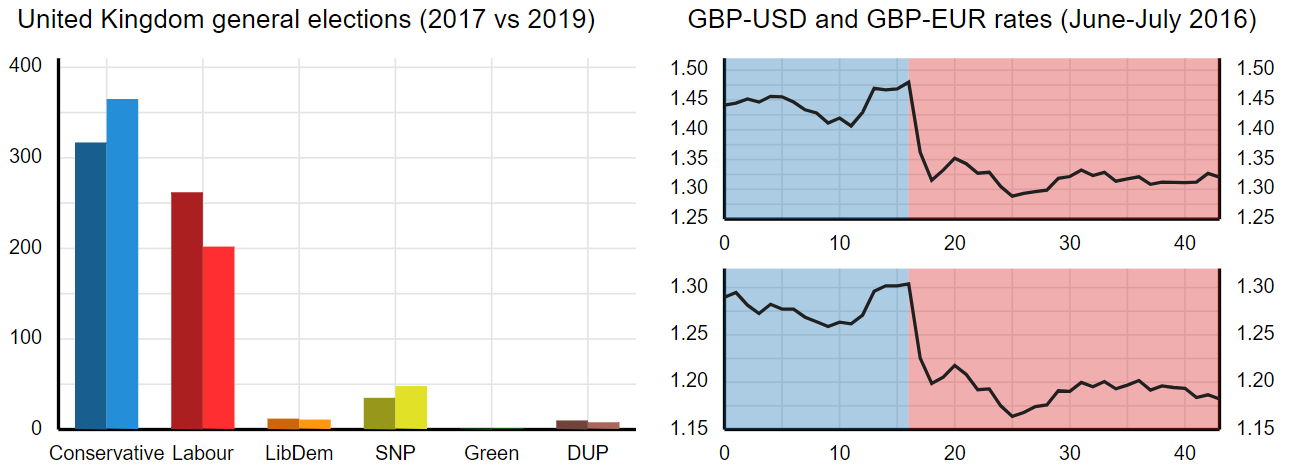
\includegraphics[scale=0.55]{figures/charts}
  \vspace{0.25em}
  \caption{Two charts about UK politics: Comparison of election results from 2017 and 2019 (left)
  and GBP/USD exchange rate with highlighted areas before and after the 23 June 2016 Brexit vote.}
  \label{fig:charts}
\end{figure}

What would an elegant functional approach to data visualization look like? A functional programmer
would want a domain-specific language that has a small number of primitives that allow us to define
high level abstractions such as a bar chart and that uses domain values such as the exchange
rate, rather than pixels, in its basic building blocks.

As is often the case with domain-specific languages, finding the right primitives is more of an art
than science. For this reason, we present our solution, a library named Compost, as a functional pearl.
We hope to convince the reader that Compost is elegant and we illustrate this with a wide range
of examples. Compost has a number of specific desirable properties:

\begin{itemize}
\item Concepts such as bar charts, line charts or charts with aligned
  axes are all expressed in terms of more primitive building blocks using a small number of combinators.
\item The primitives are specified in domain terms. When drawing a line, the value of a \\ \Y coordinate
  is an exchange rate of 1.36 USD/GBP, not 67 pixels from the bottom.
\item Common chart types such as bar charts or line charts can be easily captured as high level
  abstractions, but many interesting custom charts can be created as well.
\item The approach can easily be integrated with the Elm architecture \cite{elm}
	to create web-based charts that involve animations or interaction with the user.
\end{itemize}
%
The presentation in this paper focuses on explaining the primitives and combinators of the
domain-specific language. We outline the structure of an implementation, but omit the details; filling
those in merely requires careful thinking about geometry and projections.

Compost is available as open-source at \urrl{http://compostjs.github.io}. It is implemented in F\#,
but is available as a plain JavaScript library thanks to the Fable F\# to JavaScript compiler.
The core logic consists of 800 lines of code and depends on the virtual-dom
library (\urrl{http://npmjs.com/package/virtual-dom}) for the
implementation of the interactive features, meaking it easily portable to other functional
programming languages.

\section{Basic charts: Overlaying chart primitives}
We introduce individual features of the Compost library gradually. The first important aspect of
Compost is that properties of shapes are defined in terms of domain-specific values. In this
section, we explain what this means and then use domain-specific values to specify the core part of the
UK election results bar chart.

\begin{figure}[t]
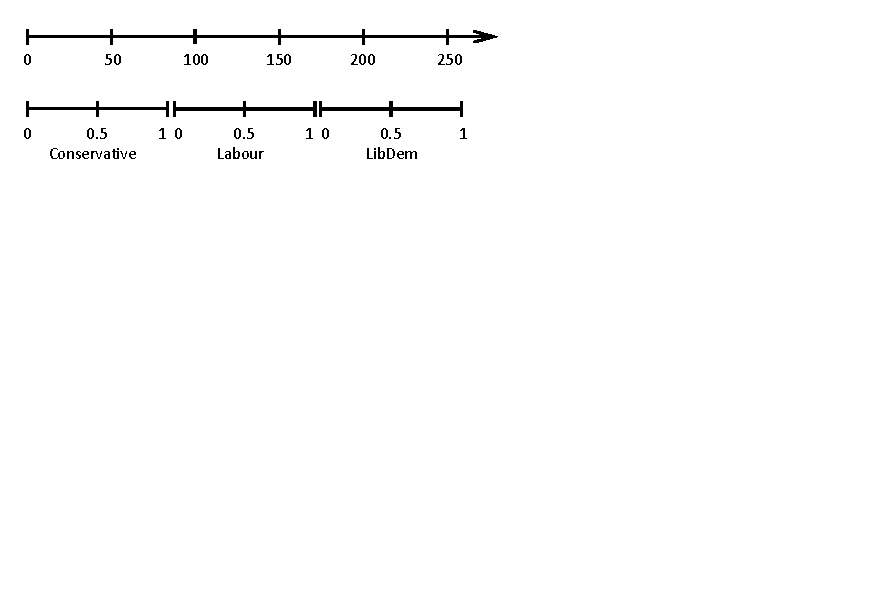
\includegraphics[scale=1,trim={0cm 6.9cm 6cm 0cm},clip]{figures/values.pdf}
\caption{On a continuous scale (above), an exact position is determined by a number.
  On a categorical scale (below), an exact position is determined by the category and a
  number between 0 and 1.}
\label{fig:scales}
\end{figure}

\subsection{Domain-specific values}

In the election results chart in Figure~\ref{fig:charts} (left), the \X axis shows categorical
values representing the political parties such as \strf{Conservative} or \strf{Labour}. The
\Y axis shows numerical values representing the number of seats won such as $\num{365}$ MPs.
When creating data visualizations, those are the values that the user needs to specify. This is
akin to most high-level charting libraries such as Google Charts, but in contrast with more
flexible libraries like D3.

Our design focuses on two-dimensional charts with \X and \Y axes. Values mapped to those axes
can be either categorical (e.g.~political parties, countries) or continuous
(e.g.~number of votes, exchange rates). The mapping from categorical and continuous values
to positions on the chart is done automatically. We discuss this in Section~\ref{sec:basic-scales}.

For example, in the UK election results chart, the \X axis is categorical. The library automatically
divides the available space between the six categorical values (political parties). The value
\strf{Green} does not determine an exact position on the axis, but rather a range. To determine
an exact position, we also need to attach a value between $\num{0}$ and $\num{1}$ to the
categorical value. This identifies a relative position in the available range.

Figure~\ref{fig:scales} illustrates the two kinds of values using the axes from the UK
election results chart. In Figure~\ref{fig:shape}, we define a value $v$ as either a continuous value
$\kvd{cont}~n$ containing any number $n$ or a categorical value $\kvd{cat}~c, r$ consisting
of a categorical value $c$ and a number $r$ between $0$ and $1$. As discussed in
Section~\ref{sec:basic-types}, continuous and categorical values can also be annotated with
units of measure to make the values more descriptive.
%
\begin{figure}
\begin{equation*}
\begin{array}{llcl}
\textit{Category} & c\\
\textit{Ratio} & r\\
\textit{Number} & n\\
\textit{Text} & t \\
\textit{Color} & \gamma \\
\textit{Value} & v & = & \kvd{cat}~c, r \\
&   & | & \kvd{cont}~n
\end{array}
\begin{array}{lrcl}
\textit{Shape} & s & = &\kvd{line}~\gamma, [\,v_{x1}, v_{y1}, \ldots, v_{xn}, v_{yn}\,]\\
&  & | & \kvd{fill}~\gamma, [\,v_{x1}, v_{y1}, \ldots, v_{xn}, v_{yn}\,] \\
&  & | & \kvd{text}~\gamma, v_x, v_y, t \\
&  & | & \kvd{bubble}~\gamma, v_x, v_y, n_w, n_h \\
&  & | & \kvd{overlay}~[\,s_1, \ldots, s_n\,] \\
&  & | &\kvd{axis}_{l/r/t/b}~s\\
&  & | &\kvd{padding}~n_t,n_r,n_b,n_l,s\\
\end{array}
\end{equation*}
\caption{Core primitives of the Compost domain-specific language. Values $v$ are either categorical
  or continuous; a shape $s$ is then defined as a simple recursive algebraic data type.}
\label{fig:shape}
\end{figure}

\subsection{Basic primitives and combinators}
\label{sec:basic-primitives}

Compost is an embedded domain-specific language, implemented as a set of functions. In the
subsequent code samples, we will use color to distinguish primitives of the Compost language,
such as \kvd{overlay} or \kvd{cat} from primitives of the host language such as \fkvd{let} or
\fkvd{for}.

A chart element is represented by a shape $s$, as defined in Figure~\ref{fig:shape}.
A primitive shape can be a text label, a line connecting a list of points, a filled polygon
defined by a list of points or a bubble at a given point with a given width and height.
The position of points is specified by \X and \Y coordinates, which can be either categorical or
continuous values. For text, line, polygon and bubble, we also include a parameter $\gamma$
that specifies the element color. The width and height of a bubble is given in pixels rather than
in domain units.

Figure~\ref{fig:shape} also defines three combinators. The most important is $\kvd{overlay}$,
which overlays given shapes. When doing this, Compost infers the range of values on the \X and \Y
axes and calculates suitable projections using a method discussed in the next
section. The $\kvd{padding}$ combinator adds padding around a specified shape and $\kvd{axis}$ adds
an axis showing the inferred scale on the left, right, top or bottom of a given shape.
Using those primitives, we can construct the simple UK election results bar chart in Figure~\ref{fig:simple} (left):

\begin{equation*}
\begin{array}{l}
\fkvd{let}~\ident{conservative},~\ident{labour}~=\\
\quad \kvd{fill}~\strf{\#0000ff},
 ~[\;\,(\kvd{cat}~\strf{Conservative}, \num{0}), (\kvd{cont}~\num{0}), (\kvd{cat}~\strf{Conservative}, \num{0}), (\kvd{cont}~\num{365}),\\
\hspace{6.7em}\;(\kvd{cat}~\strf{Conservative}, \num{1}), (\kvd{cont}~\num{365}), (\kvd{cat}~\strf{Conservative}, \num{1}), (\kvd{cont}~\num{0})\;\,],\\
\quad \kvd{fill}~\strf{\#ff0000},
 ~[\;\,(\kvd{cat}~\strf{Labour}, \num{0}), (\kvd{cont}~\num{0}), (\kvd{cat}~\strf{Labour}, \num{0}), (\kvd{cont}~\num{202}),\\
\hspace{6.7em}\;(\kvd{cat}~\strf{Labour}, \num{1}), (\kvd{cont}~\num{202}), (\kvd{cat}~\strf{Labour}, \num{1}), (\kvd{cont}~\num{0})\,\;]\\[0.5em]
\kvd{axis}_l~(\kvd{axis}_b~(\kvd{overlay}~[~\ident{conservative}, \ident{labour}~]))\\
\end{array}
\end{equation*}

\vspace{-0.25em}
\noindent
We use the \fkvd{let} construct of the host functional language to structure the code. The chart
specification overlays two bars of different colors and then adds axes to the bottom and left of the chart.
The two bars are filled rectangles defined using four corner points. The \Y
coordinates are specified as continuous values, while the \X coordinates are categorical. For
the Conservative party, two of the points have the \Y coordinate set to $\kvd{cont}~\num{0}$ (bottom of the bar)
and two have the \Y coordinate set to $\kvd{cont}~\num{365}$ (top of the bar). The two \X coordinates
are the start and the end of the range allocated for the \strf{Conservative} category,
i.e.~$\kvd{cat}~\strf{Conservative}, \num{0}$ on the left and $\kvd{cat}~\strf{Conservative}, \num{1}$
on the right.

\begin{figure}
  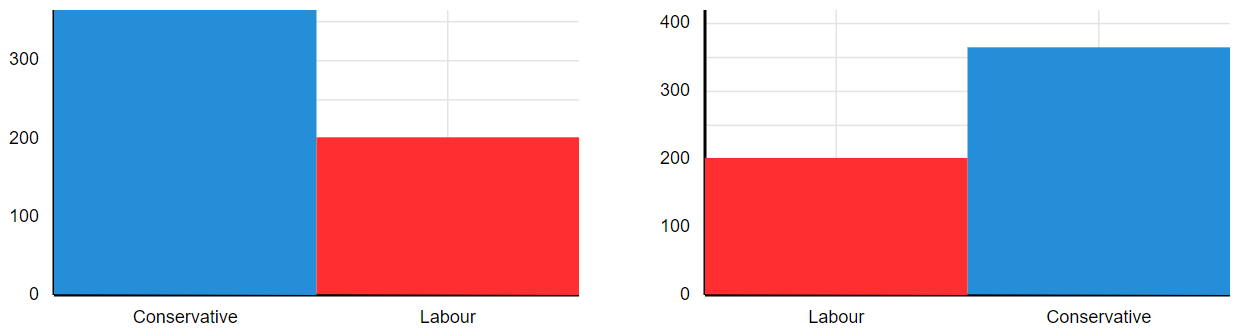
\includegraphics[scale=0.55]{figures/simple}
  \vspace{0.25em}
  \caption{Simple chart showing the UK election results; using automatically inferred scales (left)
    and using rounded Y scale and explicitly defined (reordered) X scale (right).}
  \label{fig:simple}
  \vspace{-1.5em}
\end{figure}

Extending the snippet to generate a grouped bar chart that shows two results
for each party as in Figure~\ref{fig:charts} is not much harder. Given a party $p$, we need to
generate two rectangles, one with \X coordinates $\kvd{cat}~p, 0$ and $\kvd{cat}~p, 0.5$
and the other with \X coordinates $\kvd{cat}~p, 0.5$ and $\kvd{cat}~p, 1$.
In the following snippet, we use a \fkvd{for} comprehension to generate the list. All remaining
constructs are primitives of the Compost domain-specific language. Assuming \ident{elections} is a
list of election results containing a five-element tuple consisting of a party name, colors for
2017 and 2019 and results for 2017 and 2019 we create the chart using:
%
\begin{equation*}
\begin{array}{l}
  \kvd{axis}_l~(\kvd{axis}_b~(\kvd{overlay}~[\\
  \quad \fkvd{for}~\ident{party}, \ident{clr17}, \ident{clr19}, \ident{mp17}, \ident{mp19}~\fkvd{in}~\ident{elections}~\rightarrow\\
  \quad\quad \kvd{padding}~0,10,0,10,\,\kvd{overlay}~[\\
  \quad\quad\quad \kvd{fill}~\ident{clr17},~[\,(\kvd{cat}~\ident{party}, \num{0}), (\kvd{cont}~\num{0}), (\kvd{cat}~\ident{party}, \num{0}), (\kvd{cont}~\ident{mp17}),\\
  \quad\quad\quad \hspace{4.08em}           ~(\kvd{cat}~\ident{party}, \num{0.5}), (\kvd{cont}~\ident{mp17}), (\kvd{cat}~\ident{party}, \num{0.5}), (\kvd{cont}~\num{0}) \,], \\
  \quad\quad\quad \kvd{fill}~\ident{clr19},~[\,(\kvd{cat}~\ident{party}, \num{0.5}), (\kvd{cont}~\num{0}), (\kvd{cat}~\ident{party}, \num{0.5}), (\kvd{cont}~\ident{mp19}),\\
  \quad\quad\quad \hspace{4.08em}           ~(\kvd{cat}~\ident{party}, \num{1}), (\kvd{cont}~\ident{mp19}), (\kvd{cat}~\ident{party}, \num{1}), (\kvd{cont}~\num{0})\,]~~]~~]\,)\,)\\
\end{array}
\end{equation*}

\vspace{-0.5em}
\noindent
Aside from iterating over all available parties and splitting the bar, the example also adds padding
around the bars, which is specified in pixels. A similar
result could be be achieved by drawing a bar using a range from $\num{0.05}$ to $\num{0.5}$, but
specifying padding precisely in pixels is sometimes preferable.
The chart is still missing a title, which we add in Section~\ref{sec:abstractions}.

\subsection{Choosing the level of language abstraction}
\label{sec:basic-level}

Perhaps the most important aspect of the design of any domain-specific language is the level
of abstraction it uses. The bar chart example discussed in the previous section illustrates
the choice made in Compost. On the one hand, Compost gives us flexibility by letting us
compose charts from shapes. On the other hand, Compost limits what we can do by using
two-dimensional space with positions determined by categorical or continuous values.
In other words, the Compost design lies in the middle of a broader spectrum.

An example of a more general domain-specific language is the Pan language \cite{fun} for producing
images. Pan represents images as functions from a 2D point to a color. This makes it possible to
create powerful combinators, e.g.~polar image transformation, but it makes it harder
to express logic important for charting, e.g.~automatic alignment of shapes defined in terms
of categorical values. Compost makes it easy to put two bars side-by-side in a
bar chart, but harder to define generic combinators for aligning images.

An example of a less general domain-specific language is the Haskell Chart library \cite{hcharts}.
Haskell Chart provides a wide range of plots (such as lines, candles, areas, points, error bars, pies, etc.),
but those can only be composed in limited ways by overlaying them or arranging them in a grid.
The language is closer to the domain of the most common applications, but it places more
restrictions on what can be expressed.

The design of the Compost domain-specific language aims to capture the key principles shared
by most charts, but avoid using a long list of different plot types. Different types of charts
are all produced by composing shapes, but the ways in which shapes can be composed and transformed
are limited to those that are needed for typical charts. We discuss the limitations of this
approach in more detail in Section~\ref{sec:limits}.

\subsection{Inferring scales and projections}
\label{sec:basic-scales}

We follow the terminology of Vega \cite{vega} and use the term \emph{scale} to refer to the mapping of
values to positions on a screen; a \emph{coordinate} is a value representing a position on a
scale and the term \emph{axis} is used to refer to the visual representation of a scale.

Scales are an important concept in Compost.
When composing shapes using the \kvd{overlay} primitive, the user does not need to specify how
to position the child elements relatively to each other. The Compost library positions the elements
automatically. This is done in two steps. During pre-processing, Compost infers the scales for
\X and \Y axes. A scale represents the range of values that needs to fit in the space available for
the chart. When rendering a shape, Compost projects domain-specific values to the available screen
space based on the inferred scale. A scale $l$ is defined in Figure~\ref{fig:scale}.
%
A continuous scale is defined by a minimal and maximal value that need to be mapped to the
available chart space. A categorical scale is defined by a list of individual categorical values.
Note that we do not need minimal and maximal ratios of the used categorical values as Compost
will use equal space for each category, regardless of where in this space a shape needs to
appear.

Scale inference is done by a simple recursive function that walks over the given shape and
constructs two scales for the \X and \Y axis, using the \X and \Y coordinates that appear in the shape.
Most of the work is done by a simple helper function that takes two scales, $l_1$~and $l_2$,
and produces a new scale that represents the union of the two:

\begin{equation*}
\begin{array}{l}
\ident{union}~(\kvd{continuous}~n_l, n_h)~(\kvd{continuous}~n'_l, n'_h) =\\
\qquad\kvd{continuous}~\min(n_l, n'_l), \max(n_h, n'_h)\\[0.5em]
\ident{union}~(\kvd{categorical}~[\,c_1, \ldots, c_p\,])~(\kvd{categorical}~[\,c'_1, \ldots, c'_q\,]) =\\
\qquad \kvd{categorical}~[\,c_1, \ldots, c_p\,] \;@\; [\,c'_i~|~ \forall i\in 1\ldots q, \nexists j. c_j = c'_i \;]
\end{array}
\end{equation*}

\vspace{-0.5em}
\noindent
When unioning two continuous scales, the minimum and maximum of the resulting scale is the smallest
and largest of the two minimums and maximums, respectively. When unioning two categorical scales,
we take all values of the first scale and append all values of the second scale that do not appear
in the first one. Note that this means that the order of categorical values in a scale depends on
the order in which they appear in the shape. (A possible improvement to Compost would be to support
ordinal values, which are categorical values with a well-defined ordering.) It is also worth noting
that a categorical scale cannot be combined with a continuous scale. In other words, mixing
categorical and continuous values in a single scale results in an error.

The scales inferred during pre-processing are later used when rendering a shape.
We discuss the implementation in Section~\ref{sec:impl}. The key operation is projection
which, given a coordinate, a scale and an area on the screen, produces a position on
the screen. For a continuous scale, the projection is a linear transformation. For
categorical scale with $k$ values, we split the available chart space into $k$ equally sized
regions and then map a categorical value $\kvd{cat}~c, r$ to the region corresponding to $c$
according to the ratio $r$.

\begin{figure}
\vspace{-0.5em}
\begin{equation*}
\begin{array}{rcl}
\textit{Scale}~~~l & = & \kvd{continuous}~n_{min}, n_{max} \lsep \kvd{categorical}~[\,c_1, \ldots, c_k\,]
\end{array}
\end{equation*}
\vspace{-1em}
\caption{A scale $l$ can be continuous, defined by a range, or categorical, defined by a list of values.}
\label{fig:scale}
\vspace{-1em}
\end{figure}


\subsection{Types and units of measure}
\label{sec:basic-types}

We introduce the Compost domain-specific language as untyped, but there are some obvious ways in
which types can make composing charts in Compost safer. First, a type representing a shape could
specify whether the \X and \Y axes represent categorical or continuous values. This would rule out
mixing of different values on a single scale and guarantee that the \ident{union} operation,
sketched in the previous section, is never called in a way leading to an undefined result.
Second, the type of values mapped to an axis could be further annotated with units of measure
\cite{units}. Using the F\# notation where $n\langl u\rangl$ is a number $n$ with unit $u$,
an axis containing a value $\kvd{cont}~\num{317}\langl \ident{mp}\rangl$ would then be incompatible
with an axis containing a value $\kvd{cont}~\num{1.32}\langl \ident{gbp}/\ident{usd}\rangl$.

We only outline the type system here. There are two kinds of types; $\sigma$ is a type of values
and $\tau$ is a type of shapes. Assuming $u$ denotes a unit of measure, the types are defined as:
%
\begin{equation*}
\begin{array}{rcl}
\sigma & = & \kvd{Cat}~u \lsep \kvd{Cont}~u
\end{array}
\qquad\qquad
\begin{array}{rcl}
\tau & = & \kvd{Shape}~\sigma_x, \sigma_y \\
\end{array}
\end{equation*}

\vspace{-1.25em}
\noindent
Correspondingly, there are two kinds of typing judgements; $v\vdash \sigma$ indicates the type of a
value, while $s\vdash \tau$ indicates the type of a shape. The typing rules for two of the
basic chart primitives, \kvd{line} and \kvd{overlay} look as follows:
%
\begin{equation*}
\inference
  {v_{xi} \vdash \sigma_x & v_{yi} \vdash \sigma_y}
  {\kvd{line}~\gamma, [\,v_{x1}, v_{y1}, \ldots, v_{xn}, v_{yn}\,] \vdash \kvd{Shape}~\sigma_x, \sigma_y}
\qquad
\inference
  {s_i \vdash \kvd{Shape}~\sigma_x, \sigma_y}
  {\kvd{overlay}~[\,s_1, \ldots, s_n\,] \vdash \kvd{Shape}~\sigma_x, \sigma_y}
\end{equation*}

\vspace{-0.5em}
\noindent
The rule for \kvd{line} ensures that all X and Y values have the same types, $\sigma_x$ and $\sigma_y$,
respectively and infers $\kvd{Shape}~\sigma_x, \sigma_y$ as the type of the shape. The rule for
\kvd{overlay} ensures that all composed shapes have the same type, including the type of \X and \Y scales.

\begin{figure}
\begin{equation*}
\begin{array}{rclcl}
\textit{Shape}~~~s & = & \kvd{roundScale}_{x/y} s      &|& \kvd{nest}_{x/y}~v_{min}, v_{max}, s \\
   & | & \kvd{explicitScale}_{x/y}~l, s &|&  (\ldots)
\end{array}
\end{equation*}
\caption{Additional combinators for controlling and nesting scales, extending earlier definition of $s$.}
\label{fig:control}
\end{figure}

\section{Advanced charts: Controlling scale composition}
\label{sec:fancy}

Most charts have one \X and one \Y scale that are determined by the values the chart shows,
but there are interesting exceptions. The chart in Figure~\ref{fig:charts} (right)
has two different \Y axes, one for GBP/USD and one for GBP/EUR. In the next two sections, we look at
three combinators that control the scale inference process and what flexibility this enables.

\subsection{Defining nice scale ranges}

The automatic scale inference often results in scales where the maximum is a non-round number.
This leads to charts that fully utilise the available space, but may not be easy to read.
The first two primitives, shown in Figure~\ref{fig:control} (left) allow the chart designer
to adjust the automatically inferred range of scales.
The operations can be applied to either the \X scale or the \Y scale, which is indicated by the
$x/y$ subscript. The \kvd{roundScale} primitive takes the inferred \X or \Y scale of the shape $s$
and, if it is a continuous scale, rounds its minimal and maximal values to a ``nice'' number.
For example, if a continuous scale has minimum $\num{0}$ and maximum $\num{365}$, the resulting
scale would have a maximum $\num{400}$. For categorical scale, the operation does not have any effect.
The \kvd{explicitScale} operation replaces the inferred scale with an explicitly
provided scale (the type of the inferred scale has to match with the type of the explicitly given
scale). For example, the chart in Figure~\ref{fig:simple} (right) is constructed using the
following code (reusing the \ident{conservative} and \ident{labour} variables defined earlier):
%
\begin{equation*}
\begin{array}{l}
\kvd{axis}_l~(\kvd{axis}_b~(\kvd{roundScale}_y~(\kvd{explicitScale}_x~(\kvd{categorical}~[\,\strf{Labour},\strf{Conservative}\,]),\\
\qquad \kvd{overlay}~[~\ident{conservative}, \ident{labour}~]~)))\\
\end{array}
\end{equation*}
\vspace{-0.75em}

\noindent
Reading the code from the inside out, the snippet first overlays the two coloured bars defined
earlier; it then replaces the X axis with an explicitly given one that changes the order of the
values. As a result, the bar for \strf{Labour} will appear on the left, even though the value
comes later in the list of overlaid chart elements.

The code next uses \kvd{roundScale} to automatically round the minimum and maximum of the
continuous Y scale (showing the total number of seats). Finally, we add axes around the shape,
producing a usual labelled chart.  It is worth noting that \kvd{axis} and \kvd{roundScale}
could be implemented as derived operations; \kvd{roundScale} would need to infer the scale of
the nested shape and then insert \kvd{explicitScale} with a rounded number; \kvd{axis}
would also need to infer the scales and then generates labels and lines in suitable locations.

\subsection{Nested scales}

The most interesting primitive for controlling scale composition
is $\kvd{nest}_{x/y}$. As with other primitives like \kvd{padding}, the primitive takes a shape
with some additional parameters and defines a new shape.
Its behaviour is similar to that of the SVG viewport \cite{svg}.
The \kvd{nest} primitive takes two values, $v_{min}, v_{max}$ and a shape $s$ as arguments and
nests the scale of the shape $s$ inside the region defined by $v_{min}, v_{max}$.
When inferring scales of shapes, the scale of $\kvd{nest}_{x/y}~v_{min}, v_{max}, s$ will be a
categorical or continuous scale constructed from the values $v_{min}$ and $v_{max}$, regardless
of the values that are used inside the shape $s$. The chart space between $v_{max}$ and $v_{min}$
will then be used to render the nested shape $s$ using its inferred scale. In other words, the
operation defines a virtual coordinate system that exists only inside the newly created shape,
but is invisible to anything outside of the shape.
An example of nesting is shown in Figure~\ref{fig:nesting}.
Here, a chart with a continuous scale from $\num{1.1}$ to $\num{1.4}$ (e.g.~GBP/EUR exchange rates)
is nested in the left half of another chart, which has a continuous scale from $\num{0}$ to $\num{100}$.

\begin{figure}
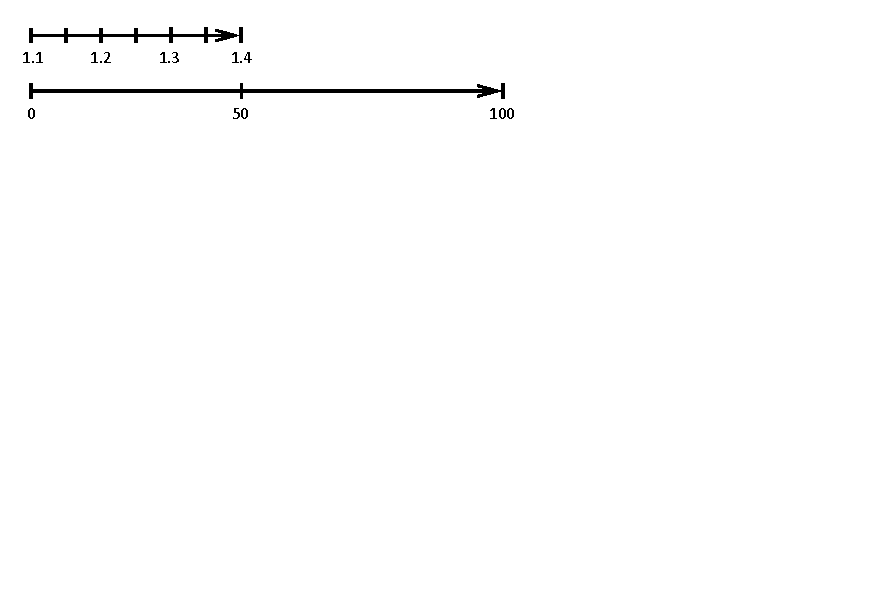
\includegraphics[scale=1,trim={0cm 7.5cm 6cm 0cm},clip]{figures/nest}
\caption{A continuous scale with values from $0$ to $6$, nested in another scale.}
\label{fig:nesting}
\end{figure}

The nesting of scales can be used in a variety of ways. For example, to nest a scatter plot
showing individual data points inside a bar of a histogram, we would use $\kvd{cat}~\strf{ABC}, 0$
and $\kvd{cat}~\strf{ABC}, 1$ as the points that define the start and the end of the region. A simpler
use case for the combinator is showing multiple charts in a single view. For example, the motivating example
in Figure~\ref{fig:charts} (right) compares aligned line charts of exchange rates for two
different currencies. Assuming \ident{gbpusd} and \ident{gbpeur} are lists containing days as \X
values and exchange rates as \Y values, we can construct a simple chart with two line charts,
shown in Figure~\ref{fig:lines} (left), using:
%
\begin{equation*}
\begin{array}{l}
\kvd{overlay}~[~
\kvd{nest}_y~(\kvd{cont}~\num{0}),(\kvd{cont}~\num{50}), (\kvd{axis}_l~(\kvd{axis}_r~(\kvd{axis}_b~(\kvd{line}~\strf{\#202020}~\ident{gbpusd}))))\\
\hspace{3.68em} \kvd{nest}_y~(\kvd{cont}~\num{50}),(\kvd{cont}~\num{100}), (\kvd{axis}_l~(\kvd{axis}_r~(\kvd{axis}_b~(\kvd{line}~\strf{\#202020}~\ident{gbpeur}))))~]\\
\end{array}
\end{equation*}

\vspace{-0.5em}
\noindent
In this example, the \X scale shows the days of the year. This scale is shared by both of the charts.
Indeed, if data was only available for the second half of the month for one of the charts,
we would want the line to start in the middle of the chart. However, the \Y scale needs to be
separate for each of the charts. To achieve this, we use $\kvd{nest}_y$. The scale of the inner
shapes is continuous, from the minimal to the maximal exchange rate for a given period. The
outer scale is determined by the explicitly defined points. For the upper chart, these are
$\kvd{cont}~\num{0}$ and $\kvd{cont}~\num{50}$; for the lower chart, these are
$\kvd{cont}~\num{50}$ and $\kvd{cont}~\num{100}$. The continuous values define a scale that only
contain two shapes -- one in the upper half, one in the lower half -- and so the three numbers could
have equally been, for example, $\num{0},\num{1}, \num{2}$. The outer scale used here is
synthetic and it is not aligned with other chart elements. A chart that does not have synthetic
outer scale is pairplot, discussed in the next section.

\begin{figure}
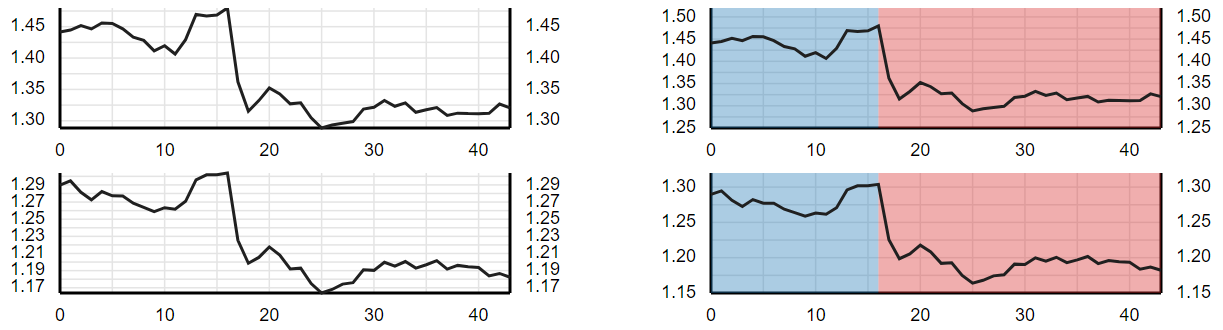
\includegraphics[scale=0.57]{figures/lines}
\vspace{0.25em}
\caption{Two charts showing currency exchange rates with a shared X scale and separate Y scales.}
\label{fig:lines}
\end{figure}

For completeness, the following code snippet shows how to construct the full currency exchange
rate chart shown in Figure~\ref{fig:lines} (right), including the blue and red background:
%
\begin{equation*}
\begin{array}{l}
\fkvd{let}~\ident{xrate}~(\ident{lo}, \ident{hi})~\ident{rates}~=\kvd{overlay}~[\\
\quad \kvd{fill}~\strf{\#1F77B460}, [\;\,\kvd{cont}~\num{0}, \kvd{cont}~\ident{lo}, \kvd{cont}~\num{16}, \kvd{cont}~\ident{lo}, \kvd{cont}~\num{16}, \kvd{cont}~\ident{hi}, \kvd{cont}~\num{0}, \kvd{cont}~\ident{hi}\;],\\
\quad \kvd{fill}~\strf{\#D6272860}, [\;\,\kvd{cont}~\num{16}, \kvd{cont}~\ident{lo}, \kvd{cont}~\num{44}, \kvd{cont}~\ident{lo}, \kvd{cont}~\num{44}, \kvd{cont}~\ident{hi}, \kvd{cont}~\num{16}, \kvd{cont}~\ident{hi}\;],\\
\quad \kvd{line}~\strf{\#202020}~\ident{rates}~]\\[0.5em]
\kvd{overlay}~[~
\kvd{nest}_y~(\kvd{cont}~\num{0}),(\kvd{cont}~\num{50}), (\kvd{axis}_l~(\kvd{axis}_r~(\kvd{axis}_b~(\ident{xrate}~(\num{1.25}, \num{1.50})~\ident{gbpusd}))))\\
\hspace{3.68em} \kvd{nest}_y~(\kvd{cont}~\num{50}),(\kvd{cont}~\num{100}), (\kvd{axis}_l~(\kvd{axis}_r~(\kvd{axis}_b~(\ident{xrate}~(\num{1.15}, \num{1.30})~\ident{gbpeur}))))~]\\
\end{array}
\end{equation*}

\noindent
Here, we use the \fkvd{let} binding of the host language to define a function that takes
the data \ident{rates} together with the minimum and maximum. This is used for drawing
two filled rectangles, covering the first 16 days of the view in blue and the rest in red.
The shapes combined using \kvd{overlay} are rendered in the order in which they appear and so
the line shape is last, so that it appears above the background.

\section{Standard charts: Defining new abstractions}
\label{sec:abstractions}

The functional domain-specific language design makes it easy to define high-level chart features
and chart types, known from standard charting libraries, using the low-level primitives of the
core language. To illustrate this, we give two examples.

First, one last remaining feature of the two charts in Figure~\ref{fig:charts} is a chart title.
This can be added to any chart using the following derived combinator:
%
\begin{equation*}
\begin{array}{l}
\fkvd{let}~\ident{title}~t~s~=\kvd{overlay}~[\\
\quad \kvd{nest}_x~(\kvd{cont}~\num{0}), (\kvd{cont}~\num{100}),
  (\kvd{nest}_y~(\kvd{cont}~\num{0}), (\kvd{cont}~\num{15}), \\
\quad\quad \kvd{explicitScale}_x~(\kvd{continuous}~\num{0},\num{100}),~(\kvd{explicitScale}_y~(\kvd{continuous}~\num{0},\num{100}),\\
\quad\qquad \kvd{text}~\strf{\#000000}, (\kvd{cont}~\num{50}), (\kvd{cont}~\num{50}),~t)~)\\
\quad \kvd{nest}_x~(\kvd{cont}~\num{0}), (\kvd{cont}~\num{100}),
  (\kvd{nest}_y~(\kvd{cont}~\num{15}), (\kvd{cont}~\num{100}),~s)~]
\end{array}
\end{equation*}

\vspace{-0.5em}
\noindent
We use \fkvd{let} in the host language to define \ident{title} as a function taking a title $t$ and
a shape $s$. It overlays two shapes. To position the title above the chart, the~first
shape has an outer \Y scale $\kvd{continuous}~\num{0},\num{15}$ while the second has an outer \Y scale
$\kvd{continuous}~\num{15},\num{100}$. Similarly, the outer \X scale of both is $\kvd{continuous}~\num{0},\num{100}$.
These are defined using $\kvd{nest}_{x/y}$.

\begin{figure}
  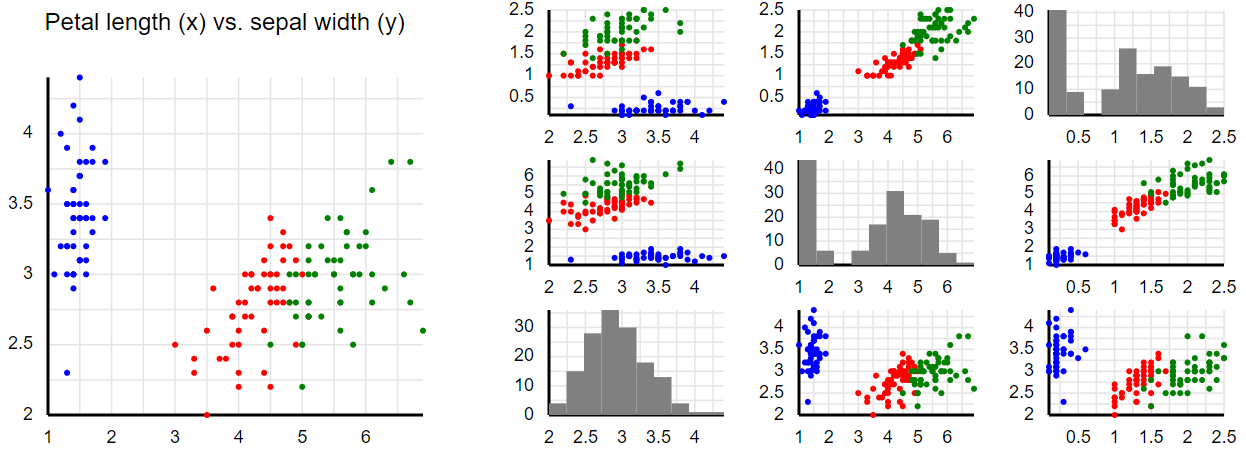
\includegraphics[scale=0.57]{figures/standard}
  \vspace{0.25em}
  \caption{Sample charts built using derived abstractions; a scatter plot visualizing the Iris dataset with a title (left) and a pairplot comparing two Iris features (right).}
  \label{fig:standard}
\end{figure}

The second shape simply wraps the specified chart $s$ to which we are attaching the title. The first
positions the text title in the middle of the available space. To do so, we explicitly set the \X and
\Y scales inside the upper shape to continuous scales from $\num{0}$ to $\num{100}$ and then position
the text label in the middle, at a point $(\kvd{cont}~\num{50}), (\kvd{cont}~\num{50})$. We assume
that the \kvd{text} primitive centers the text, although the actual implementation also allows the
user to specify horizontal and vertical alignment.
Figure~\ref{fig:standard} (left) shows a sample scatter plot chart with a title created using the
\ident{title} combinator.

A more complex chart that can be composed using the Compost primitives is pairplot from the seaborn
library \cite{seaborn}. Pairplot visualizes pairwise relationships between features of a dataset.
An example using three features (sepal width, petal width, petal length) from the Iris dataset is shown
in Figure~\ref{fig:standard} (right).
A pairplot draws a grid of charts, each visualizing the relationship between two numerical features. For distinct
features, pairplot shows a scatter plot using one feature for \X values and the other for \Y values.
When the features are the same (the diagonal), it draws a histogram of the feature values.
A categorical feature can be used to determine the color of dots in the scatter plots.

To generate a pairplot, we use \kvd{nest} to overlay and align a grid of plots. Each of those
overlays a number of bubbles or filled shapes and adds left and bottom axis. As before, we use
\fkvd{let} to define a function and list comprehensions to generate individual chart elements.
We assume that \ident{data} is a list of rows, \ident{attrs} is a list of available attributes and
$\ident{get}~a~r$ obtains the attribute $a$ of a row $r$. We also assume the dataset contains the \str{color} attribute.
%
\begin{equation*}
\begin{array}{l}
\fkvd{let}~\ident{pairplot}~\ident{attrs}~\ident{data}~=~\kvd{overlay}~[\\
\quad \fkvd{for}~x~\fkvd{in}~\ident{attrs}~\rightarrow~\fkvd{for}~y~\fkvd{in}~\ident{attrs}~\rightarrow\\
\qquad \kvd{nest}_x~(\kvd{cat}~x, 0), (\kvd{cat}~x, 1), (\kvd{nest}_y~(\kvd{cat}~y, 0), (\kvd{cat}~y, 1), \kvd{axis}_l~(\kvd{axis}_b\\
\quad\qquad (~\fkvd{if}~x \neq y~\fkvd{then}~\kvd{overlay}~[\;\fkvd{for}~r~\fkvd{in}~\ident{data}~\rightarrow~\\
\qquad\qquad \hspace{0.7em} \kvd{bubble}~(\ident{get}~\str{color}~r),~(\ident{get}~x~r), (\ident{get}~y~r), \num{1}, \num{1}~]\\
 \quad\qquad \hspace{0.7em} \fkvd{else}~\kvd{overlay}~[\;\fkvd{for}~x_1, x_2, y~\fkvd{in}~\ident{bins}~x~\ident{data}~\rightarrow~\\
\qquad\qquad \hspace{0.7em}  \kvd{fill}~\strf{\#808080}~[\; x_1, y, x_2, y, x_2, \num{0}, x_1, \num {0}\;]\;])))] \\
\end{array}
\end{equation*}

\vspace{-0.5em}
\noindent
As before, \kvd{nest} is essential for composing individual charts. Here, the points that determine
the locations of individual charts are categorical values defined by the attributes of the dataset.
The choice between two possible nested charts is made using the host language \fkvd{if} construct.
Scatter plots are generated by overlaying bubbles with \X and \Y coordinates obtained using $\ident{get}~x~r$
and $\ident{get}~y~r$. Histograms are composed from filled shapes. To obtain their locations, we use
a helper function $\ident{bins}~x~\ident{data}$, which returns a list of bins specified by a triple
consisting of a lower and an upper range $x_1, x_2$ and the count $y$.

The example shows that Compost is simple yet expressive. With just
a few lines of code, we are able to construct charts that, in other systems, require dedicated
libraries. The essential aspect of the language making this possible is the automatic inference
of scales and their mapping to the available space as well as the \kvd{nest} operation.


\section{Interactive charts: Domain-specific event handling}
Many data visualizations published on the web feature interactivity. Standard forms of
interactivity include animations, hover labels or zooming. More interesting custom
visualizations include ``You Draw It'' introduced by the New York Times \cite{youdraw}.
The chart shows only the first half of the data, such as a timeline, and the reader has to
guess the second half before clicking a button and seeing the actual data. Standard forms of
interactivity are often supported by high-level libraries; Google Charts supports panning
using drag \& drop, zooming to a selected chart range and animations. Custom interactivity is
typically implemented using low-level libraries such as D3, but doing so requires directly handling
JavaScript events and modifying the browser DOM.

Compost uses the Elm architecture \cite{mvu} to support interactive data visualizations.
In this model, an interactive visualization is described using a pair of user-defined types
and a pair of user-defined functions. The \emph{state} type represents the current state of what
is displayed (e.g.~animation step or selection) and the \emph{event} type represents actions that
the user can perform (e.g.~start an animation or draw a selection range). The two functions
use the state and event types. The \emph{view} function creates a chart based on the current
state and the \emph{update} function specifies how the state changes when an event occurs.

\subsection{Domain-specific events}

To support handling of mouse-based events, Compost adds three additional primitives to the definition
of shape, shown in Figure~\ref{fig:mouse}. The three new primitives make it possible to handle
three common mouse events using custom functions $\lambda x~y\rightarrow e$, specified in the
host language. The most interesting aspect is that the functions are given \X and \Y coordinates
of the event specified in the domain units of the chart. This means that if the user clicks on the
bar representing the Conservative party in a bar chart, the values might be, for example,
$\kvd{cat}~\strf{Conservative},\num{0.75}$ for \X and $\kvd{cont}~\num{120.5}$ for \Y.

\begin{figure}
\begin{equation*}
\begin{array}{rclcl}
s & = & \kvd{mouseUp}~(\lambda \,x~y \rightarrow e), s  &|& \kvd{mouseDown}~(\lambda \,x~y\rightarrow e), s  \\
    &|& \kvd{mouseMove}~(\lambda \,x~y \rightarrow e), s &|& (\ldots)
\end{array}
\end{equation*}
\caption{Additional combinators for mouse-based interaction, extending earlier definition of $s$.}
\vspace{0.5em}
\label{fig:mouse}
\end{figure}

\subsection{You Draw It data visualizations}
To illustrate building interactive data visualizations using Compost, we look at one aspect of
``You Draw It''. We want to create a bar chart where the user can use drag \& drop
to move individual bars. Figure~\ref{fig:youdraw} shows the interactive chart before and after an
interaction. The first step is to define types representing the state and events that can occur:

\noindent
\begin{equation*}
\begin{array}{lll}
\fkvd{type}~\ident{State} &\narrow{=}& \ident{bool}~*~(\ident{string}~*~\ident{int})~\ident{list}\\
\fkvd{type}~\ident{Event} &\narrow{=}& \ident{Update}~\fkvd{of}~(\ident{string}~*~\ident{int}) ~~|~~ \ident{Moving}~\fkvd{of}~\ident{bool}
\end{array}
\end{equation*}

\vspace{-0.5em}
\noindent
The state is a pair of a boolean, indicating whether the user is currently dragging, and
a list of key/value pairs, storing the number of seats for each political party. Two types of events
can occur in the visualization. First, the user may start or stop dragging, which is indicated using
$\ident{Moving}(\fkvd{true})$ and $\ident{Moving}(\fkvd{false})$, respectively. Second, the user
may change a value for a party, which is represented by the $\ident{Update}$ event.

The next part of the implementation is the \ident{update} function which takes an old state together
with an event and produces a new state:
%
\begin{equation*}
\begin{array}{l}
\fkvd{let}~\ident{update}~(\_,s)~(\ident{Moving}(m)) = m,s\\
\hspace{1.05em}~\ident{update}~(\fkvd{true},s)~(\ident{Update}(p, v)) =
%\hspace{1.05em}\qquad
  \fkvd{true}, \ident{map}~(\lambda(k, o) \rightarrow k, \fkvd{if}~k = p~\fkvd{then}~v~\fkvd{else}~o)~s\\
\hspace{1.05em}~\ident{update}~(m,s)~(\ident{Update}(\_, \_)) = m,s\\
\end{array}
\end{equation*}

\vspace{-0.5em}
\noindent
The first case handles the \ident{Moving} event, which replaces the first component of the
state tuple, i.e.~a flag indicating whether a mouse button is down.
The next two cases handle the \ident{Update} event. The event carries two values, $p, v$, which
represent the party (which bar the user is dragging) and the new value (new number of seats).
If the user is currently dragging, we replace the value associated with the party $p$ in \noindent the
list $s$ using the \ident{map} function. If the user is not currently dragging, the event is ignored.

Finally, the \ident{view} function takes the current state and builds the data visualization
using the Compost domain-specific language. In addition, it also takes a parameter \ident{trigger},
which is an effectful function of type $\ident{Event}\rightarrow\ident{unit}$ that can be used to
trigger events in handlers, registered using primitives such as \kvd{mouseMove}. The \ident{trigger}
function is provided by the Compost runtime. When it is invoked from an event handler, it takes
the current state, transforms it using the \emph{update} function, sets the new state as the
current state and invokes the \emph{view} function to display the new state.

To build the bar chart in Figure~\ref{fig:youdraw}, we use the same approach as in
Section~\ref{sec:basic-primitives}. The only addition are the event handlers registered using
\kvd{mouseMove}, \kvd{mouseUp} and \kvd{mouseDown}:
%
\begin{equation*}
\begin{array}{l}
\fkvd{let}~\ident{view}~\ident{trigger}~(\_, \ident{state})~=\\
\quad \kvd{axis}_l~(\kvd{axis}_b~(\kvd{explicitScale}_y~(\kvd{continuous}~\num{0},\num{400}),\\
\qquad (~\kvd{mouseMove}~(\lambda \,(\kvd{cat}~p,\_)~(\kvd{cont}~v)\rightarrow \ident{trigger}(\ident{Update}(p, v))),\\
\qquad (~\kvd{mouseUp}~(\lambda \,\_~\_\rightarrow \ident{trigger}(\ident{Moving}(\fkvd{true}))),\\
\qquad (~\kvd{mouseDown}~(\lambda \,\_~\_\rightarrow \ident{trigger}(\ident{Moving}(\fkvd{false}))),~\kvd{overlay}~[\\
\qquad \qquad \fkvd{for}~\ident{party}, \ident{mps}~\fkvd{in}~\ident{state}~\rightarrow~\kvd{padding}~0,10,0,10,~(\kvd{fill}~(\ident{color}~\ident{party}),\\
\qquad \qquad\quad\quad [\,(\kvd{cat}~\ident{party}, \num{0}), (\kvd{cont}~\num{0}), (\kvd{cat}~\ident{party}, \num{0}), (\kvd{cont}~\ident{mp}),\\
\qquad \qquad\quad\quad \hspace{0.38em}(\kvd{cat}~\ident{party}, \num{0.5}), (\kvd{cont}~\ident{mps}), (\kvd{cat}~\ident{party}, \num{0.5}), (\kvd{cont}~\num{0}) \,])~~])))))\\
\end{array}
\end{equation*}

When the user interacts with the visualization created using Compost, the library
translates the coordinates associated with events from pixels to domain-specific
values. In case of the above bar chart, when the user moves a mouse, the function registered
using \kvd{mouseMove} is given a categorical value $\kvd{cat}~p, r$ as the \X coordinate and
a continuous value $\kvd{cont}~v$ as the \Y coordinate. It then takes $p$, which is the name
of the party corresponding to the bar and the value $v$ corresponding to the number of seats
and triggers the $\ident{Update}(p, v)$ event to update the state. The handlers for
\kvd{mouseUp} and \kvd{mouseDown} do not use the coordinates. They simply switch the flag
indicating whether the user is currently dragging or not.

The primitives for specifying mouse event handlers can be nested or appear in multiple sub-shapes
of the composed shape. This makes it possible to attach different event handlers to different
parts of a chart and get event coordinates in local units. In case of nesting, the nested handler
will capture events that occur in the space occupied by the shape it wraps, but it will ignore
events occuring outside of this area.

The pair of functions, \ident{update} and \ident{view}, together with an initial state is
all that is needed to create an interactive data visualization. Compost calls
\ident{view} each time the state changes and uses virtual-dom to update the chart
displayed in the browser. Although creating an interactive visualization is more work than
creating a static one, the domain-specific nature of Compost is invaluable. We can
simply take the values $p$ and $v$ produced by a mouse event, use those to update the state
and then, again, render an updated chart.

\begin{figure}[t]
  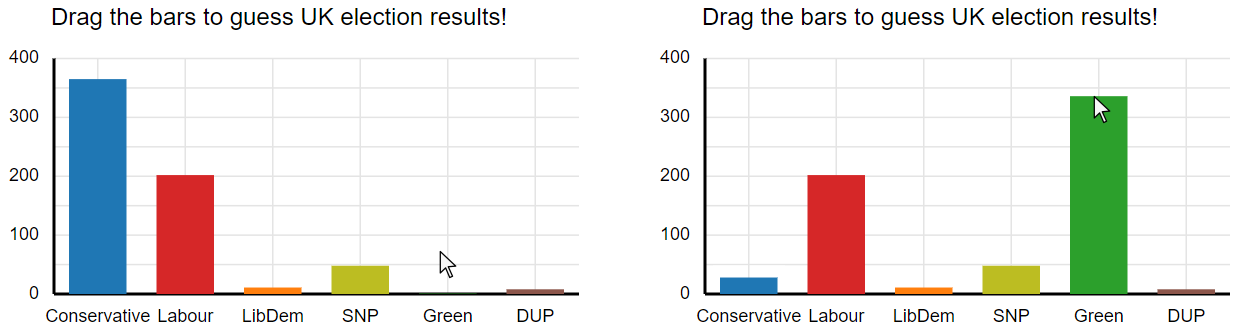
\includegraphics[scale=0.57]{figures/youdraw}
  \vspace{1em}
  \caption{Interactive ``You Draw it'' data visualization. The user moves cursor to a bar (left),
    pushes a mouse button and drags the bar to the position that they think is the correct one (right).}
  \label{fig:youdraw}
\end{figure}


\section{Implementation structure: Scale inference and rendering}
\label{sec:impl}

Compost is an open-source library, implemented in the functional language F\#. The full source
code can be found at \urrl{http://github.com/compostjs}.
As is often the case with functional domain-specific languages, the implementation is not difficult
once we find the right collection of basic primitives and the right structure for the implementation.
This largely applies to the Compost library and so we will not go into the implementation details.
It is, however, worth giving an outline of the implementation structure.

As mentioned in Section~\ref{sec:basic-scales}, the rendering of shapes proceeds in two stages.
First, the library infers the scales of a shape. When doing so, it also annotates some shapes
with additional information that is needed later for rendering. Second, the library projects
the shape onto an available space and produces the chart, represented as an SVG object.

\subsection{Inferring the scales of a shape}
\label{sec:impl-infer}

In order to render a shape, we need to know the range of values that should appear on the \X and
\Y axes. This is done by inferring a scale for each of the axes from the individual \X and \Y
coordinates that specify shape locations. As discussed earlier, a scale can be either categorical
(displaying only categorical values) or continuous (displaying only continuous values). When
inferring scales, we use two helper operations; \ident{union}, discussed earlier, combines two
scales and \ident{singleton} creates a scale from a single coordinate.

The operation that infers the scales of a shape is \ident{calculateScales}. It takes a shape
and produces a pair of \X and \Y scales, together with a transformed shape:
%
\begin{equation*}
  \ident{calculateScales} ~:~ \ident{Shape} \rightarrow (\ident{Scale}*\ident{Scale}) * \ident{Shape}
\end{equation*}

\vspace{-1.25em}
\noindent
The operation does not need to transform the shape in most cases. The exception is the
shape $\kvd{nest}_{x/y}~v_{min}, v_{max}, s$. In this case, the returned scale is based solely on the
values of $v_{min}$ and $v_{max}$. For rendering we need to keep the inferred scales of the nested
shape $s$. To do so, the operation replaces the $\kvd{nest}_{x/y}$ shape with an auxiliary shape
$\kvd{scaledNest}_{x/y}$:

\begin{equation*}
\begin{array}{rclcl}
s &=& \kvd{scaledNest}_{x/y}~v_{min},\;v_{max},\;s_{x/y},\;s &|& (\ldots)
\end{array}
\end{equation*}

\vspace{-1em}
\noindent
There are two kinds of cases handled by \ident{calculateScales}. For primitives, it constructs
a pair of scales from individual coordinates using \ident{union} and \ident{singleton}. For
shapes containing a sub-shape, the operation calculates the scales of a sub-shape recursively
and then adapts those somehow. To illustrate, we consider two interesting cases:
%
\begin{equation*}
\begin{array}{l}
\ident{calculateScales}~(\kvd{nest}_x~v_{min},\;v_{max},\;s) = \\
\quad\fkvd{let}~(s_x, s_y),s' = \ident{calculateScales}~s\\
\quad(\ident{union}~(\ident{singleton}~v_{min})~(\ident{singleton}~v_{max}), s_y),~\kvd{scaledNest}_x~v_{min},\;v_{max},\;s_x,\;s'\\
\\
\ident{calculateScales}~(\kvd{overlay}~l) = \\
\quad\fkvd{let}~\ident{scales},\;l'~=~\ident{unzip}~(\ident{map}~\ident{calculateScales}~l)\\
\quad\fkvd{let}~s_x,s_y~=~\ident{unzip}~\ident{scales}\\
\quad(\ident{reduce}~\ident{union}~s_x,~\ident{reduce}~\ident{union}~s_y), \kvd{overlay}~l'
\end{array}
\end{equation*}

\vspace{-0.5em}
\noindent
When calculating the scales of the $\kvd{nest}_x$, the function first calculate scales of the
sub-shape $s$ recursively. The resulting \Y scale $s_y$ is returned as the result, while the \X
scale is obtained from the two coordinates $v_{min}$ and $v_{max}$. This is also the case where
the shape is transformed and the returned $\kvd{scaledNest}_x$ shape stores the inferred \X scale
$s_x$ of the sub-shape $s$. The second example is the $\kvd{overlay}$ case which recursively
computes scales of all sub-shapes and combines those using the list folding function
\ident{reduce} with $\ident{union}$ as an argument.

\subsection{Projecting coordinates and drawing}
The key operation that needs to be performed when drawing a shape is projecting coordinates from
domain-specific values to the screen coordinates. As we draw a shape, we keep the \X and \Y scale
and the space in pixels that it should be drawn on. Initially, the \X and \Y scales are those
inferred for the entire shape and the space in pixels is $\num{0}\ldots\ident{width}$ and
$\num{0}\ldots\ident{height}$ where $\ident{width}\times\ident{height}$ is the size of the target
SVG element.

The key calculation is done by the \ident{project} function, which takes the space in pixels (as a
pair of floating-point numbers representing the range), the current scale and a domain-specific value
and produces a coordinate in pixels:
%
\begin{equation*}
\ident{project}~:~\ident{float}*\ident{float}\rightarrow \ident{Scale}\rightarrow\ident{Value} \rightarrow \ident{float}
\end{equation*}

\vspace{-1.25em}
\noindent
The function is only defined if the value and scale are compatible. As discussed in Section~\ref{sec:basic-types},
this could be guaranteed using a simple type system. If both are continuous, the
function performs a simple linear transformation. If both are categorical, the available pixel
space is divided into a equally-sized bins, one for each categorical value on the scale, and the
value is then projected into the appropriate bin.

The drawing of shapes is done by a function that takes the available area as a quadruple $(x_1, y_1), (x_2, y_2)$
together with the \X and \Y scale mapped onto the area and a shape to be drawn. The result is
a data structure representing an SVG document:
%
\begin{equation*}
\ident{drawShape}~:~(\ident{float}*\ident{float})*(\ident{float}*\ident{float}) \rightarrow \ident{Scale}*\ident{Scale}\rightarrow\ident{Shape}\rightarrow\ident{Svg}
\end{equation*}

\vspace{-1.25em}
\noindent
For primitive shapes, the operation projects the coordinates using \ident{project} and constructs
a corresponding SVG document. For shapes with sub-shapes it calls itself recursively, possibly
with an adjusted scale or area. The two cases discussed earlier illustrate this:
%
\begin{equation*}
\begin{array}{l}
\ident{drawShape}~a~s~(\kvd{overlay}~l) = \\
\quad\ident{concat}~(\ident{map}~(\ident{drawShape}~a~s)~l)\\
\\[-0.5em]
\ident{drawShape}~((x_1, y_1), (x_2, y_2))~(s_x, s_y)~(\kvd{scaledNest}_x~v_{min},\;v_{max},\;{ns}_x,\;\ident{shape}) = \\
\quad\fkvd{let}~x_1' = \ident{project}~(x_1, x_2)~s_x~v_{min}\\
\quad\fkvd{let}~x_2' = \ident{project}~(x_1, x_2)~s_x~v_{max}\\
\quad\ident{drawShape}~((x_1', y_1), (x_2', y_2))~({ns}_x, s_y)~\ident{shape}\\
\end{array}
\end{equation*}

\vspace{-0.5em}
\noindent
When drawing \kvd{overlay}, the function draws all sub-shapes onto the same
area using the same scales and then concatenates the returned SVG components using the \ident{concat} helper.
The $\kvd{scaledNest}_x$ case is more illuminating. Here, we first
use \ident{project} to find the range $x_1', x_2'$ corresponding to the domain-values
$v_{min},v_{max}$. This defines the area corresponding to the nested scale ${ns}_x$, onto
which the \X coordinates in the sub-shape $\ident{shape}$ should be projected.
To do this, we recursively call \ident{drawShape}, but use $x_1'$ and $x_2'$ as the \X coordinates
of the target area and ${ns}_x$ as the \X scale. The \Y area and scales are propagated unchanged.

\section{Limitations and future work}
\label{sec:limits}

As discussed in Section~\ref{sec:basic-level}, the Compost library chooses a level of abstraction
that makes it possible to express a wide range of charts, but does not allow arbitrary image
manipulation. The examples discussed so far provide a good review of what can be expressed
using Compost. It is also worth considering what cannot currently be expressed. For many of the
current limitations, we also consider what additional primitive would address the problem.

\subsection{Radial charts and image transformations}
Compost cannot currently produce pie charts and other radial charts. This could be supported by
defining a primitive \kvd{polar} that renders a shape $s$ specified as a parameter using
a polar coordinate system instead of the default Cartesian system. Like the \kvd{nest} primitive,
this would create a new shape that occupies a newly defined chart region. The \kvd{polar}
primitive would make it possible to create pie charts, but also more elaborate Circos charts
used to visualize genomic data \cite{circos}.

Radial charts provide a clear motivation for supporting polar geometries, but we do not currently
expect the need for more general image transformations such as those supported by Pan \cite{fun}.
Those are useful for producing visually appealing images, but may not be necessary for data
visualization. Arguably, we also do not expect the need for more general layout combinators such
as \ident{above} or \ident{besides}  \cite{monoids}. Those can be expressed elegantly using image transformations.
In Compost, we can achieve similar effect using \kvd{nest} and \kvd{explicitScale}, as shown when
definining \ident{title} in Section~\ref{sec:abstractions}.


\subsection{Combinations and transformations of scales}

Another area in which Compost could be extended is to allow more flexible handling of scales.
Currently, categorical scales are mapped to bins of equal size and continuous scales are mapped
using a linear transformation. The current design does not make it possible to use logarithmic
scale or, for example, contracted axis where a sub-range of values in the middle is omitted.
Both of these could be supported if Compost allowed the user to specify a custom value
transformation function.

Another interesting challenge is to allow overlaying of charts with multiple scales. This can
currently be done by using \kvd{overlay} together with \kvd{nest}. However, a more principled
approach would be to allow the user to specify multiple, possibly named, scales for each shape.
The \ident{calculateScales} operation discussed in Section~\ref{sec:impl-infer} would then need
to return a list of scales rather than just a pair.

\subsection{Controlling visual elements of a chart}

There is also a number of occasions where the user might require more control over various
visual elements of the chart such as fonts, text alignment or visual aspects of the automatically
generated axes. The current implementation of Compost already allows control over fonts, font
sizes and text alignment, but we omit the details for brevity.

Controlling the visual aspects of axes is a more interesting problem. In fact, the
\kvd{axis} primitive described in this paper is not a primitive operation, but rather a derived
one. It is implemented by calculating the scales of the shape specified as an argument and
overlaying it with lines (for axes and grid), text elements (for labels) and adding a padding.
The current implementation does not allow much customization, but the user can look at the
implementation and easily create their own version, much like they can create their own version
of the \ident{title} operation described in Section~\ref{sec:abstractions}.

\section{Conclusions}
This paper presents a functional take on the problem of designing easy to use, but flexible
abstractions for composing data visualizations. We hope to find a sweet spot between high-level, but
inflexible approaches and low-level, but hard to use approaches.

Most work in this space is based on Grammar of Graphics \cite{grammar}, designing more or less complex and
powerful variants \cite{layered,vega-lite,vega,polaris}. In Grammar of Graphics, a chart is a mapping from
data to chart elements and their visual attributes. In contrast, in Compost, the mapping is
specified in the host programming language and a chart is merely a resulting data type
describing the visual elements using domain-specific primitives.

Our approach is very flexible as it lets the user compose primitive visual elements in any
way they want; it lets them define their own high-level abstractions and it also integrates well
with reactive programming architectures to support interactive data visualizations.

In this paper, we focus on presenting the core ideas behind Compost. However, much
remains to be explored, both in terms of finding the best set of primitives and in terms of
their language integration. First, we only support categorical and continuous values, but
there are also ordinal values (which cannot be compared, but can be sorted). Second, some of our
primitives, namely \kvd{axis} and \kvd{roundScale} could be implemented as derived operations, but
we treat those as built-in for simplicity. Third, we only treat \X and \Y as scales, but we could
similarly treat other visual features (colors of bars, size of bubbles) as scales, which would
allow a more high-level specification of certain charts.

\paragraph{Acknowledgements}
The Compost library is the result of my prolonged effort to create an elegant charting API for
F\#, which was supported, at various stages, by Don Syme at Microsoft Research and Howard Mansell
at BlueMountain Capital. The idea of Compost first came together in discussion with Mathias
Brandewinder and was (much much later) implemented thanks to the support of Google Digital News
Initiative and The Alan Turing Institute. The final motivation for this paper was an invitation
to talk at the LambdaDays conference in Krak\'ow and the positive comments from the attendees.
Finally, the anonymous referees provided valuable feedback that made this a better paper.

\bibliographystyle{jfp}
\bibliography{paper}

\end{document}
%
